\documentclass{article}


% Things to import:
\usepackage{tikz}
\usetikzlibrary{shapes}



\begin{document}
% Used to export it as an image too: (Sourcecode is from here: https://tex.stackexchange.com/a/299008)
\hoffset=-1in\voffset=-1in\setbox0\vbox{
	
\centering
	

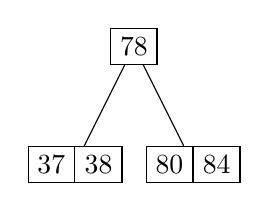
\begin{tikzpicture}
\tikzstyle{bplus}=[rectangle split, rectangle split horizontal,rectangle split ignore empty parts,draw, align=center]
\tikzstyle{every node}=[bplus]

\node {78}
child {node {37 \nodepart{two} 38}}
child {node {80 \nodepart{two} 84}}
;
\end{tikzpicture}

\bigbreak

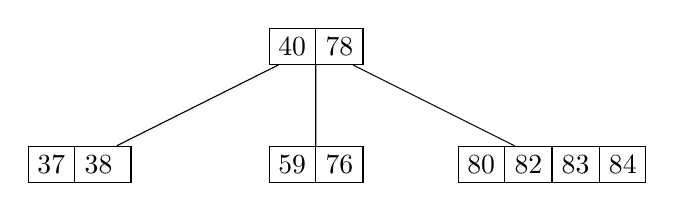
\begin{tikzpicture}
\tikzstyle{bplus}=[rectangle split, rectangle split horizontal,rectangle split ignore empty parts,draw, align=center]
\tikzstyle{every node}=[bplus]
\tikzstyle{level 1}=[sibling distance=30mm]

\node {40  \nodepart{two} 78}
child {node {37 \nodepart{two} 38 }}
child {node {59 \nodepart{two} 76}}
child {node {80 \nodepart{two} 82 \nodepart{three} 83 \nodepart{four} 84}}
;
\end{tikzpicture}

\bigbreak

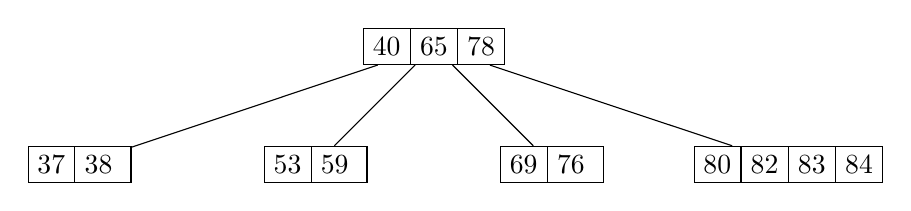
\begin{tikzpicture}
\tikzstyle{bplus}=[rectangle split, rectangle split horizontal,rectangle split ignore empty parts,draw, align=center]
\tikzstyle{every node}=[bplus]
\tikzstyle{level 1}=[sibling distance=30mm]

\node {40 \nodepart{two} 65 \nodepart{three} 78}
child {node {37 \nodepart{two} 38 }}
child {node {53 \nodepart{two} 59 }}
child {node {69 \nodepart{two} 76 }}
child {node {80 \nodepart{two} 82 \nodepart{three} 83 \nodepart{four} 84}}
;
\end{tikzpicture}

\bigbreak

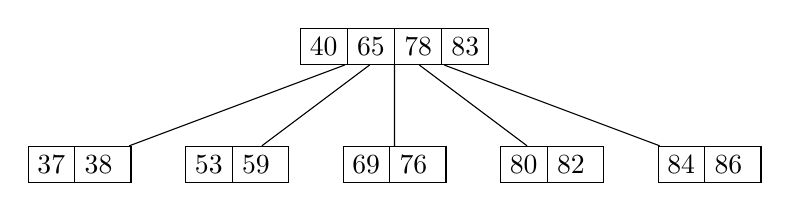
\begin{tikzpicture}
\tikzstyle{bplus}=[rectangle split, rectangle split horizontal,rectangle split ignore empty parts,draw, align=center]
\tikzstyle{every node}=[bplus]
\tikzstyle{level 1}=[sibling distance=20mm]

\node {40 \nodepart{two} 65 \nodepart{three} 78 \nodepart{four} 83}
child {node {37 \nodepart{two} 38 }}
child {node {53 \nodepart{two} 59 }}
child {node {69 \nodepart{two} 76 }}
child {node {80 \nodepart{two} 82 }}
child {node {84 \nodepart{two} 86 }}
;
\end{tikzpicture}

\bigbreak

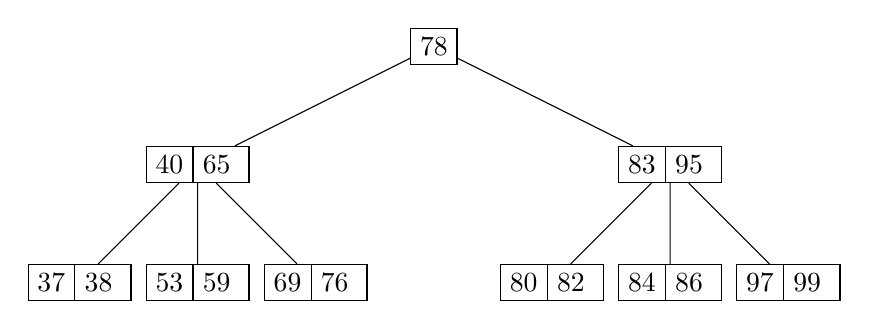
\begin{tikzpicture}
\tikzstyle{bplus}=[rectangle split, rectangle split horizontal,rectangle split ignore empty parts,draw, align=center]
\tikzstyle{every node}=[bplus]
\tikzstyle{level 1}=[sibling distance=60mm]
\tikzstyle{level 2}=[sibling distance=15mm]
\tikzstyle{level 3}=[sibling distance=20mm]

\node {78}
child {node {40 \nodepart{two} 65 }
	child {node {37 \nodepart{two} 38 }}
	child {node {53 \nodepart{two} 59 }}
	child {node {69 \nodepart{two} 76 }}
}
child {node {83 \nodepart{two} 95 }
	child {node {80 \nodepart{two} 82 }}
	child {node {84 \nodepart{two} 86 }}
	child {node {97 \nodepart{two} 99 }}
}
;
\end{tikzpicture}

	
}\pdfpageheight=\dimexpr\ht0+\dp0\relax\pdfpagewidth=\wd0\shipout\box0\stop